\documentclass[10pt,twocolumn,letterpaper]{article}

\usepackage{cvpr}
\usepackage{times}
\usepackage{epsfig}
\usepackage{graphicx}
\usepackage{amsmath}
\usepackage{amssymb}
\usepackage{subfigure}
\usepackage{epstopdf}
\usepackage{multirow}

% Include other packages here, before hyperref.

% If you comment hyperref and then uncomment it, you should delete
% egpaper.aux before re-running latex.  (Or just hit 'q' on the first latex
% run, let it finish, and you should be clear).
\usepackage[breaklinks=true,bookmarks=false]{hyperref}

\cvprfinalcopy % *** Uncomment this line for the final submission

\def\cvprPaperID{****} % *** Enter the CVPR Paper ID here
\def\httilde{\mbox{\tt\raisebox{-.5ex}{\symbol{126}}}}

% Pages are numbered in submission mode, and unnumbered in camera-ready
%\ifcvprfinal\pagestyle{empty}\fi
\setcounter{page}{1}
\begin{document}

%%%%%%%%% TITLE
\title{CMPE 264 - Project Assignment 1}

\author{Yanan Xie\\
{\tt\small yaxie@ucsc.edu}
% For a paper whose authors are all at the same institution,
% omit the following lines up until the closing ``}''.
% Additional authors and addresses can be added with ``\and'',
% just like the second author.
% To save space, use either the email address or home page, not both
\and
Ziqiang Wang\\
{\tt\small secondauthor@i2.org}
}

\maketitle
%\thispagestyle{empty}

%%%%%%%%% ABSTRACT

%%%%%%%%% BODY TEXT
\section{Camera radiometric calibration}
\label{sec:crc}

In this section, we describe how we take pictures and estimate the relationship between $B$ and $T$.

%-------------------------------------------------------------------------
\subsection{Taking pictures}

In order to simulate a surface with uniform radiance, we put a scratch paper on the table. Then, we took 9 pictures with a Canon 5D Mark II(DSLR) and a 40mm lens. A tripod was utilized to stabilize the camera. ISO was set to 100. F-number of the lens was set to 4. The exposure times of those 9 pictures are $1/25s$, $1/30s$, $1/40s$, $1/50s$, $1/60s$, $1/80s$, $1/100s$, $1/125s$, and $1/160s$ respectively. Pictures are all JPEG format. Figure \ref{fig:samplepicture} shows a picture taken with $T = 1/30s$ as an example. \\

Sample area was chosen to be the center of the picture with a size $100\times 100$. As shown in figure \ref{fig:sampler}, \ref{fig:sampleg} and \ref{fig:sampleb}, the sampled areas are not saturated in any channels. And the strips confirmed that the pictures were taken very stably.

\begin{figure}[bhp]
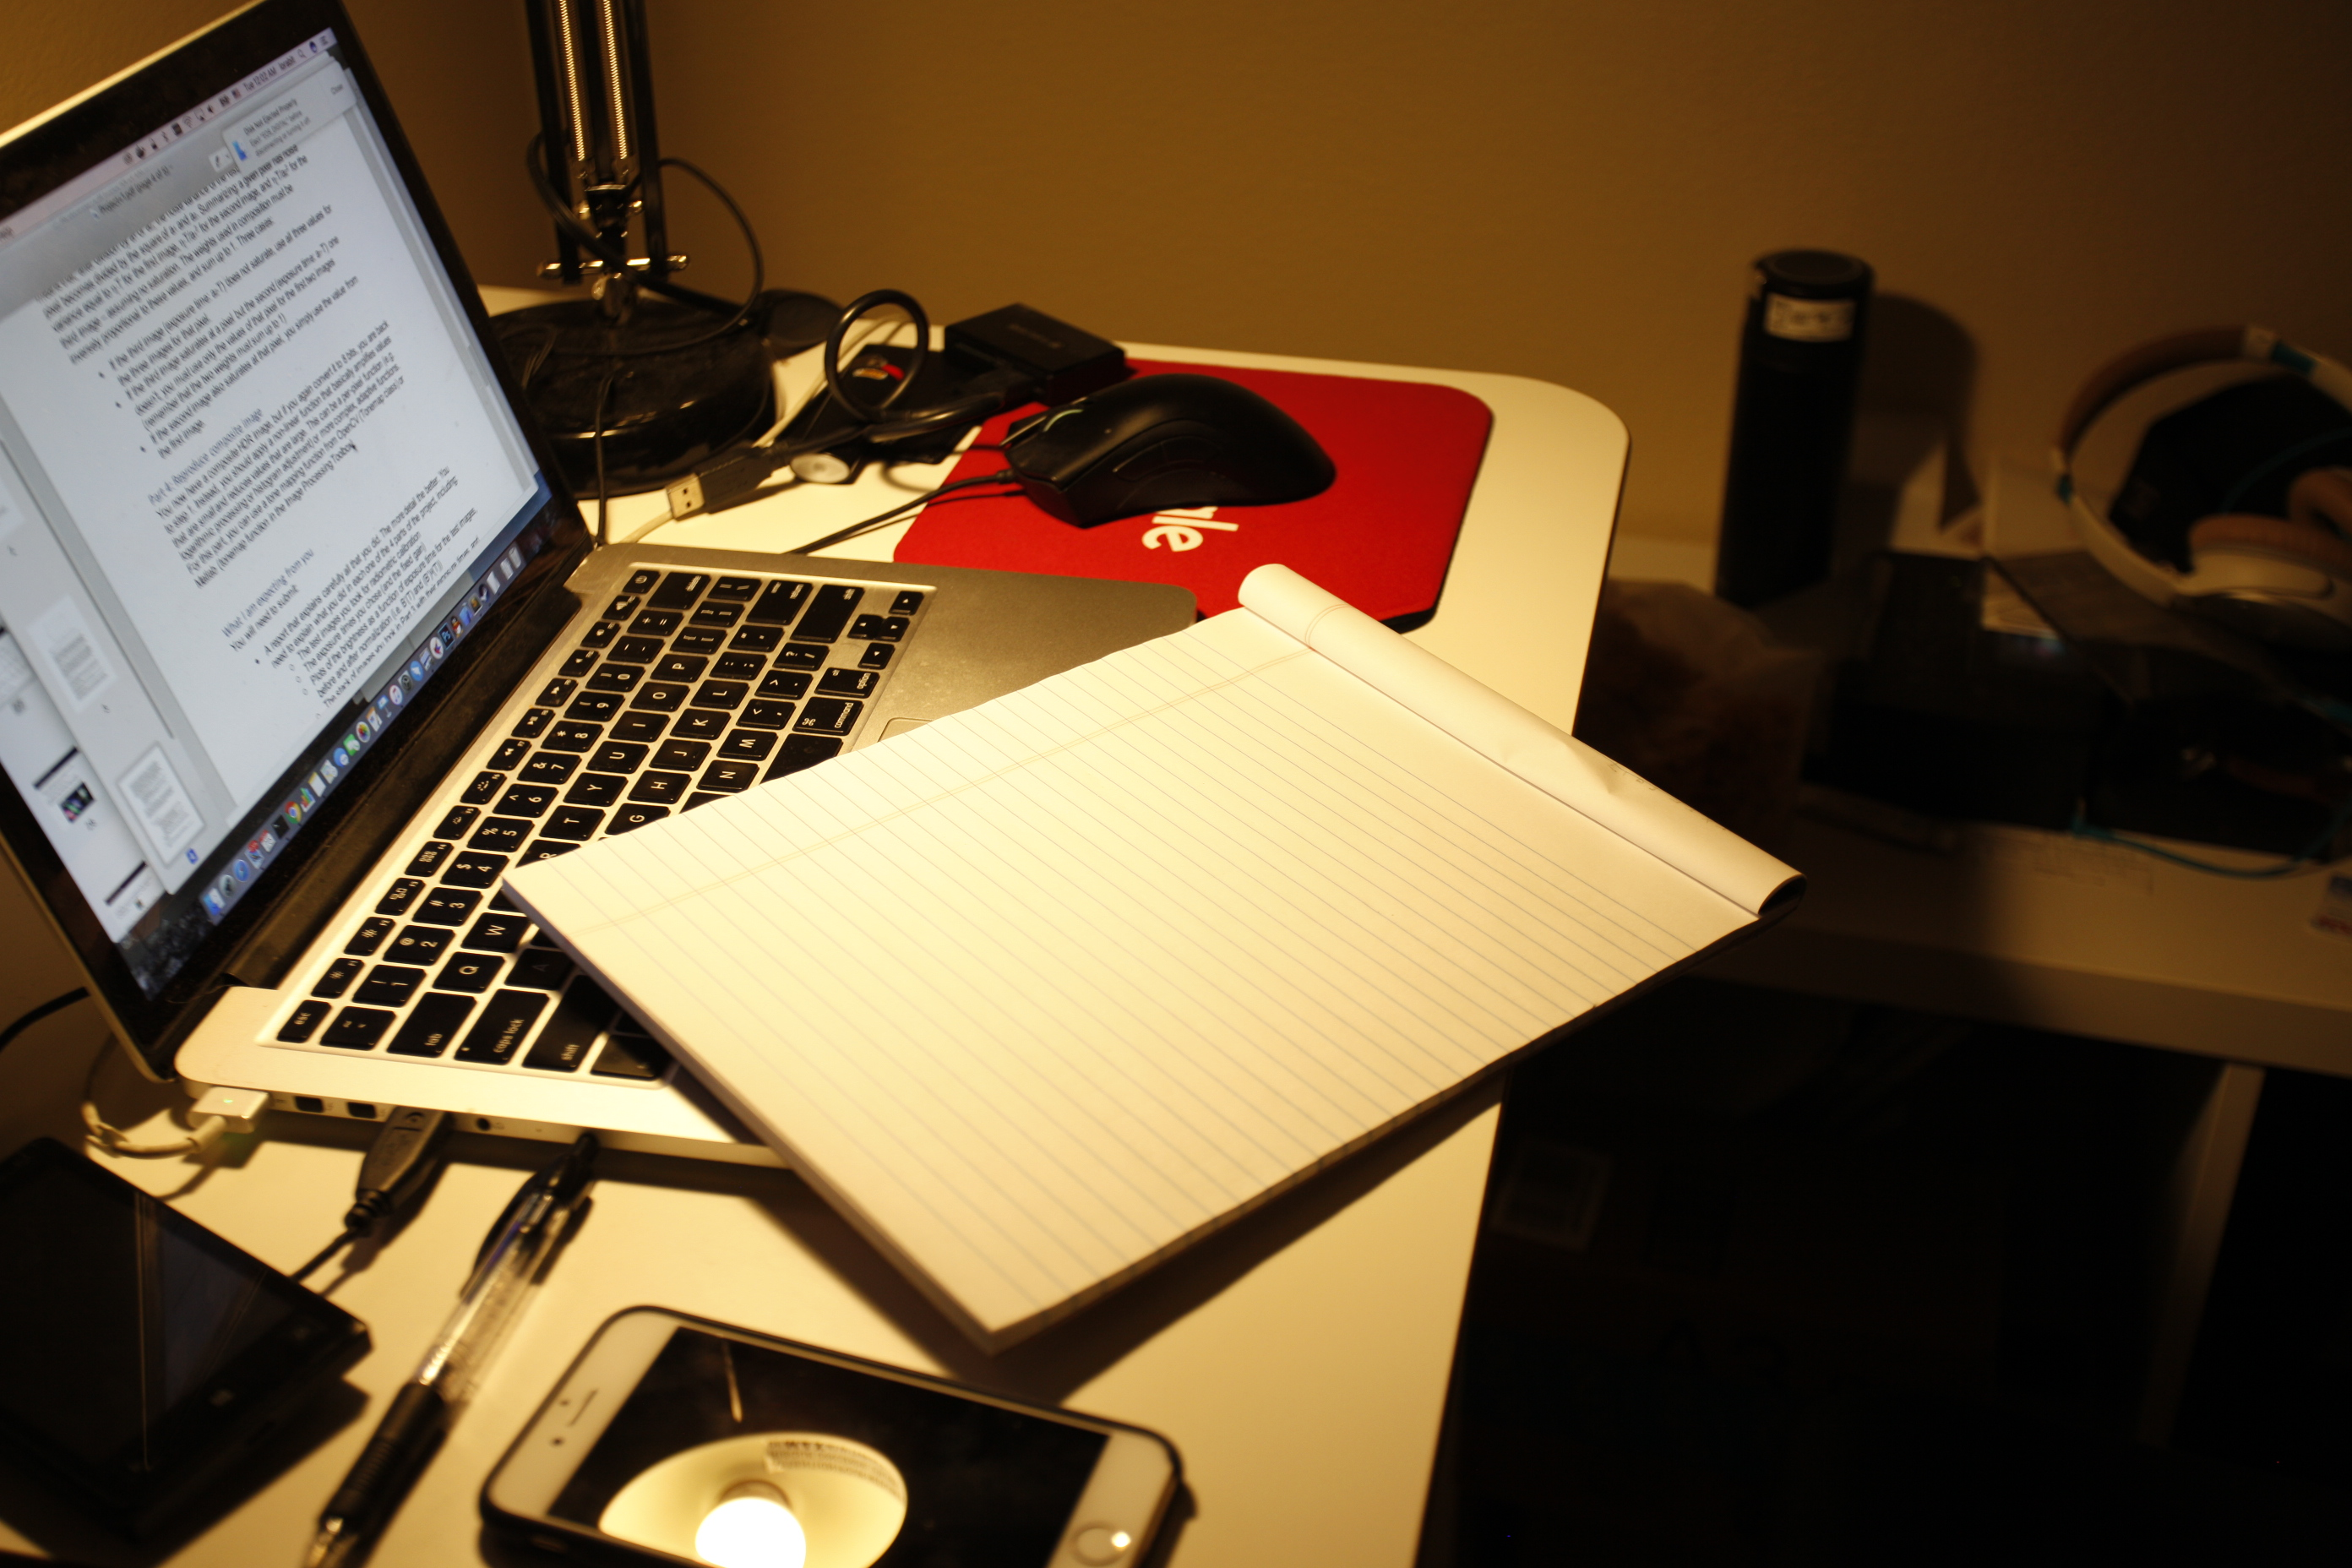
\includegraphics[width=\columnwidth]{images/_MG_6277}
\caption{Picture took with $T = 1/30s$}

\label{fig:samplepicture}
\end{figure}


\begin{figure}[t]
\centering
\subfigure[$T=1/160s$]{

\includegraphics[width=.3\columnwidth]{images/samples/0_2}
}
\subfigure[$T=1/125s$]{

\includegraphics[width=.3\columnwidth]{images/samples/1_2}
}
\subfigure[$T=1/100s$]{

\includegraphics[width=.3\columnwidth]{images/samples/2_2}
}
\subfigure[$T=1/80s$]{

\includegraphics[width=.3\columnwidth]{images/samples/3_2}
}
\subfigure[$T=1/60s$]{

\includegraphics[width=.3\columnwidth]{images/samples/4_2}
}
\subfigure[$T=1/50s$]{

\includegraphics[width=.3\columnwidth]{images/samples/5_2}
}
\subfigure[$T=1/40s$]{

\includegraphics[width=.3\columnwidth]{images/samples/6_2}
}
\subfigure[$T=1/30s$]{

\includegraphics[width=.3\columnwidth]{images/samples/7_2}
}
\subfigure[$T=1/25s$]{

\includegraphics[width=.3\columnwidth]{images/samples/8_2}
}

\caption{Sample areas of Channel R}
\label{fig:sampler}
\end{figure}

\begin{figure}[t]
\centering
\subfigure[$T=1/160s$]{

\includegraphics[width=.3\columnwidth]{images/samples/0_1}
}
\subfigure[$T=1/125s$]{

\includegraphics[width=.3\columnwidth]{images/samples/1_1}
}
\subfigure[$T=1/100s$]{

\includegraphics[width=.3\columnwidth]{images/samples/2_1}
}
\subfigure[$T=1/80s$]{

\includegraphics[width=.3\columnwidth]{images/samples/3_1}
}
\subfigure[$T=1/60s$]{

\includegraphics[width=.3\columnwidth]{images/samples/4_1}
}
\subfigure[$T=1/50s$]{

\includegraphics[width=.3\columnwidth]{images/samples/5_1}
}
\subfigure[$T=1/40s$]{

\includegraphics[width=.3\columnwidth]{images/samples/6_1}
}
\subfigure[$T=1/30s$]{

\includegraphics[width=.3\columnwidth]{images/samples/7_1}
}
\subfigure[$T=1/25s$]{

\includegraphics[width=.3\columnwidth]{images/samples/8_1}
}

\caption{Sample areas of Channel G}
\label{fig:sampleg}
\end{figure}

\begin{figure}[t]
\centering
\subfigure[$T=1/160s$]{

\includegraphics[width=.3\columnwidth]{images/samples/0_0}
}
\subfigure[$T=1/125s$]{

\includegraphics[width=.3\columnwidth]{images/samples/1_0}
}
\subfigure[$T=1/100s$]{

\includegraphics[width=.3\columnwidth]{images/samples/2_0}
}
\subfigure[$T=1/80s$]{

\includegraphics[width=.3\columnwidth]{images/samples/3_0}
}
\subfigure[$T=1/60s$]{

\includegraphics[width=.3\columnwidth]{images/samples/4_0}
}
\subfigure[$T=1/50s$]{

\includegraphics[width=.3\columnwidth]{images/samples/5_0}
}
\subfigure[$T=1/40s$]{

\includegraphics[width=.3\columnwidth]{images/samples/6_0}
}
\subfigure[$T=1/30s$]{

\includegraphics[width=.3\columnwidth]{images/samples/7_0}
}
\subfigure[$T=1/25s$]{

\includegraphics[width=.3\columnwidth]{images/samples/8_0}
}

\caption{Sample areas of Channel B}
\label{fig:sampleb}
\end{figure}

\subsection{Discovering the relation between $B$ and $T$}

$B$ is estimated by the average value of the sampled area $B'$. We calculate $B'$ in RGB channels independently in order to solve the non-linear function between $B'$ and $B$. \\

We assume $B(T) = (B'(T))^g = cETG = KT  $ following the assumption given by the instruction where $K = cEG$. By applying logarithm to both sides of the equation, we have 
$$ g\ln(B') = \ln(K) + \ln(T) $$
$$ \ln(B') = \ln(K)/g + \ln(T)/g = a + b\ln(T) $$ where $a = \ln(K)/g$ and $b=1/g$. \\

We used sklearn to estimate the coefficient of linear regression by taking $[\ln(T_i)]$ as the $X$ vector, and $[\ln(B'_i)]$ as the $Y$ vector. As shown in Table \ref{tab:linear}, the result suggests us to choose $g_R = 2.308$, $g_G = 1.962$ and $g_B = 1.484$ for RGB channels respectively. We show the $B'^g(T)$ curves before and after applied estimated $g$ in Figure \ref{fig:samplecurves}\\


\begin{table}[]
\caption{Linear regression results}
\centering
\begin{tabular}{|c|c|c|c|c|}
\hline
Channel &  $a$  &  $b$ & $g$ & mean squared error  \\
\hline

Red & 7.011 & 0.4334 & 2.308 & 0.004156 \\
\hline
Green & 7.129& 0.5097 & 1.962 & 0.002331\\
\hline
Blue & 7.297 & 0.6737 & 1.484 & 0.0008915\\
\hline

 \hline

\end{tabular}
\label{tab:linear}
\end{table}


With estimation of $g$, and given the value of $B'(T) = (KT)^{1/g}$ for some pixel, we can estimate $B'(T_{dest})$ by 
\begin{equation}
\begin{aligned}
B'(T_{dest})     &=  (KT_{dest})^{1/g}\\
            &=  (KT)^{1/g}T_{dest}^{1/g}/T^{1/g}\\
            &=  B'(T) (\frac{T_{dest}}{T})^{1/g}
\end{aligned}
\label{equ:nonlinear}
\end{equation}
for the same pixel. Also, we can estimate $B(T)$ by
\begin{equation}
\begin{aligned}
B(T)     &=  B'^g(T)
\end{aligned}.
\label{equ:linear}
\end{equation}

\begin{figure}[t]
\centering
\subfigure[Red Channel $g=1$]{
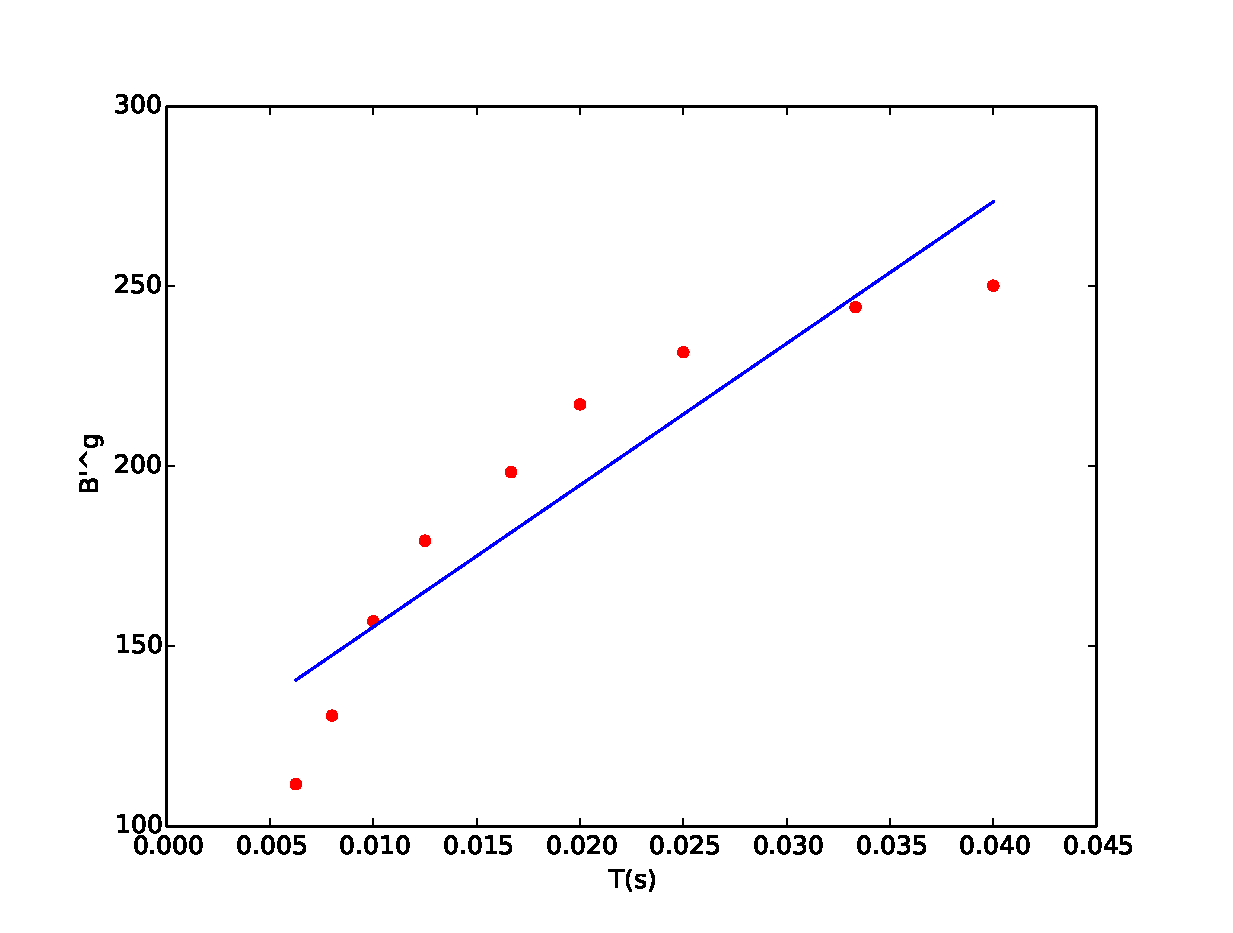
\includegraphics[width=.47\columnwidth]{images/rchannel}
}
\subfigure[Red Channel $g=2.308$]{
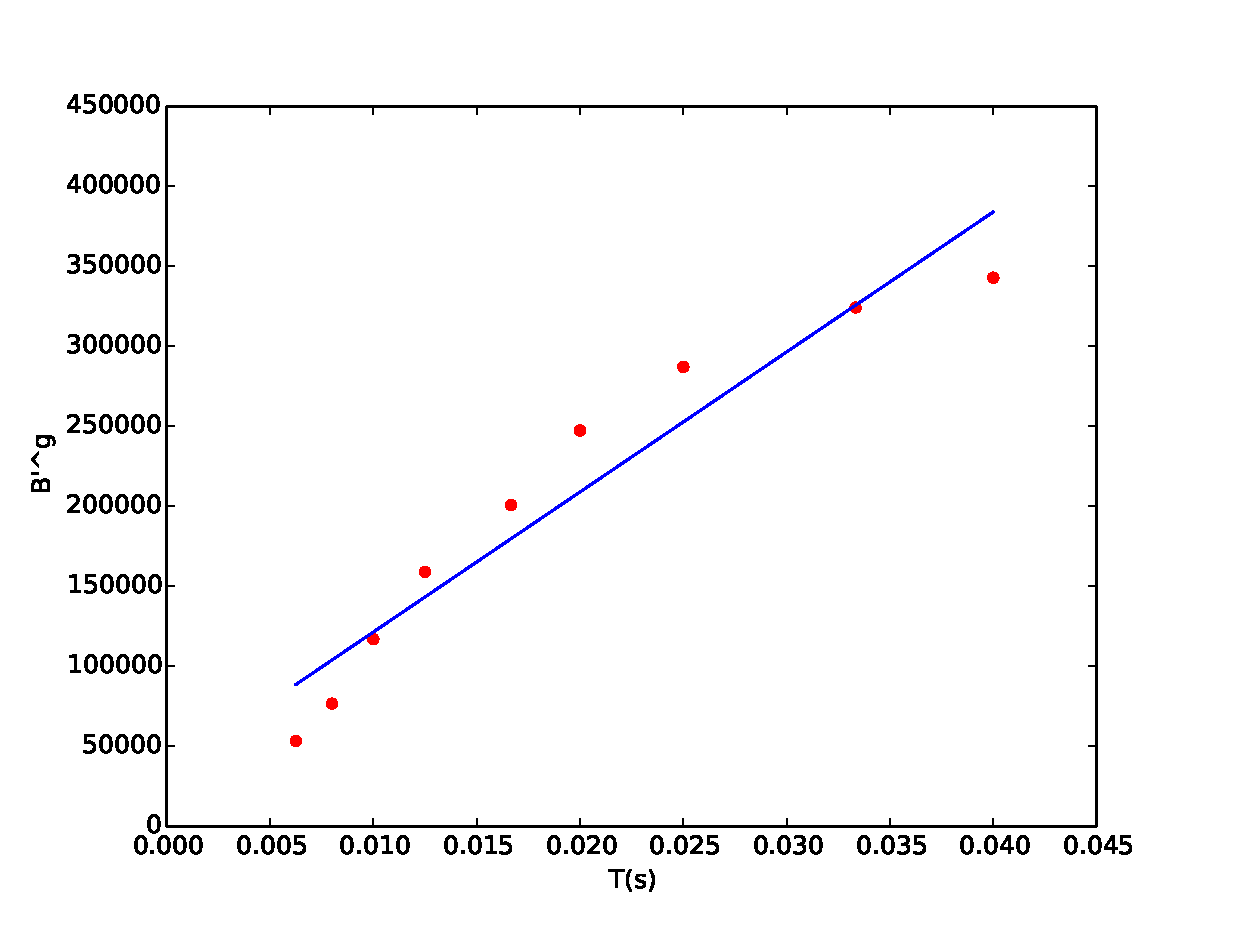
\includegraphics[width=.47\columnwidth]{images/rchannelg}
}
\subfigure[Green Channel $g=1$]{
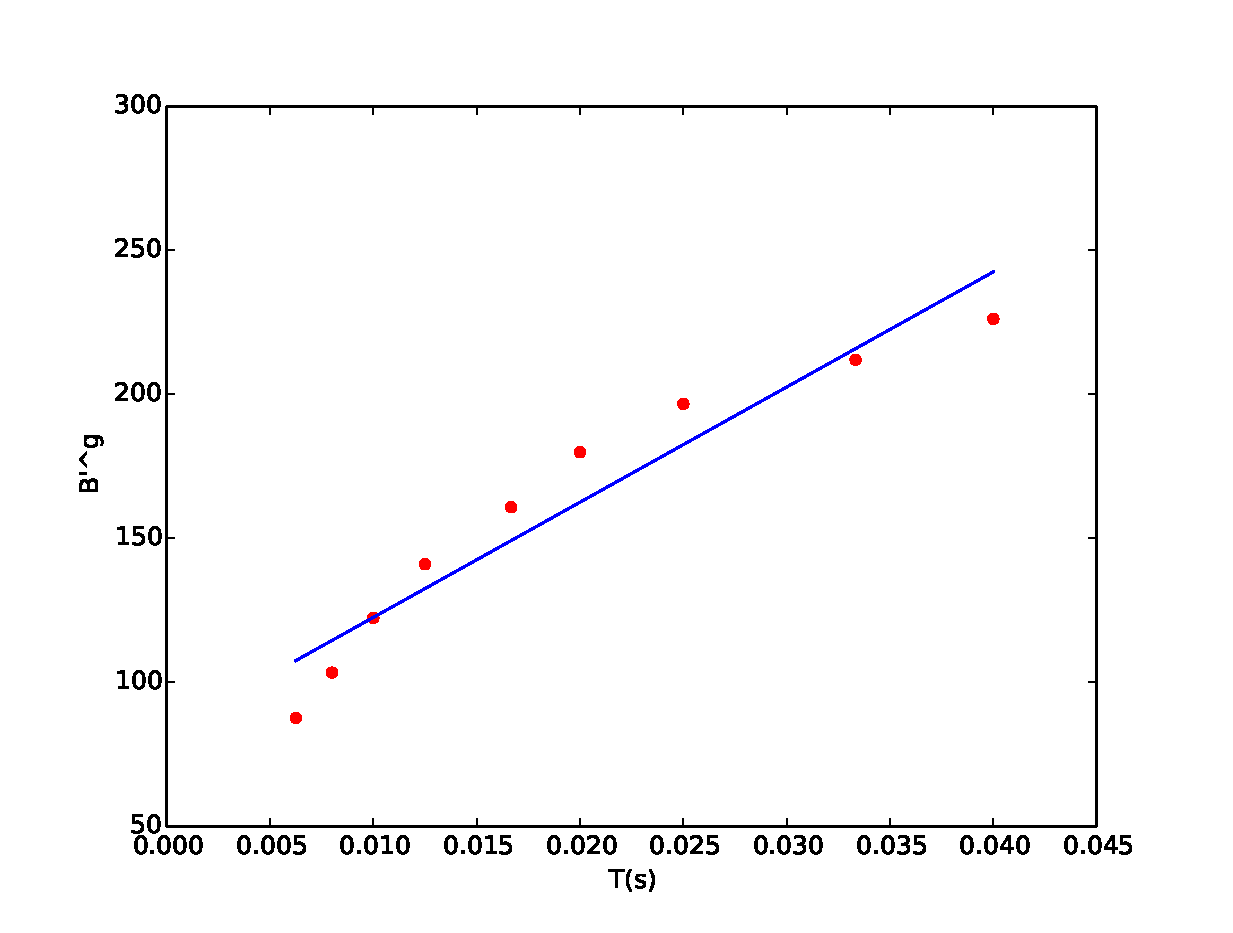
\includegraphics[width=.47\columnwidth]{images/gchannel}
}
\subfigure[Green Channel $g=1.962$]{
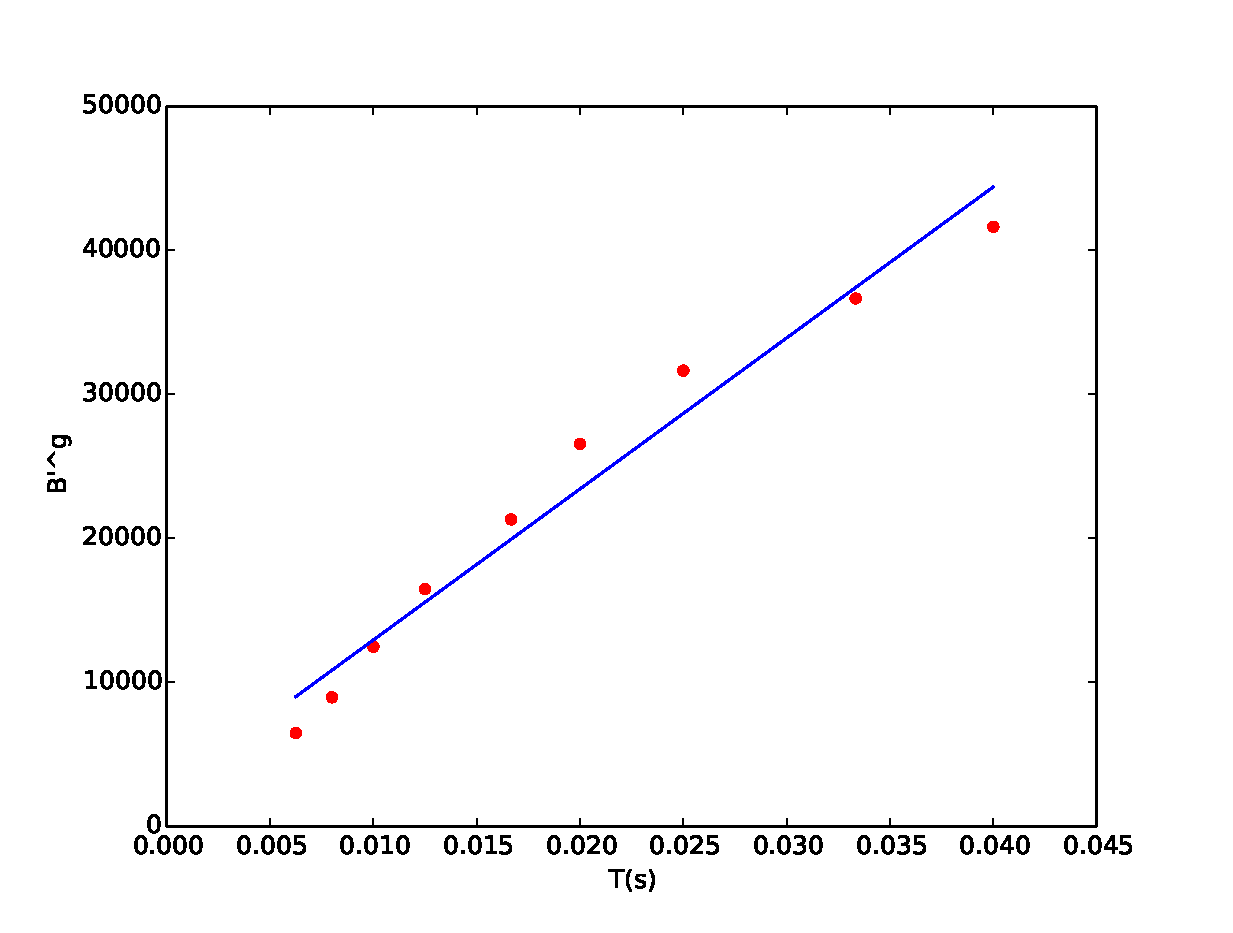
\includegraphics[width=.47\columnwidth]{images/gchannelg}
}

\subfigure[Blue Channel $g=1$]{
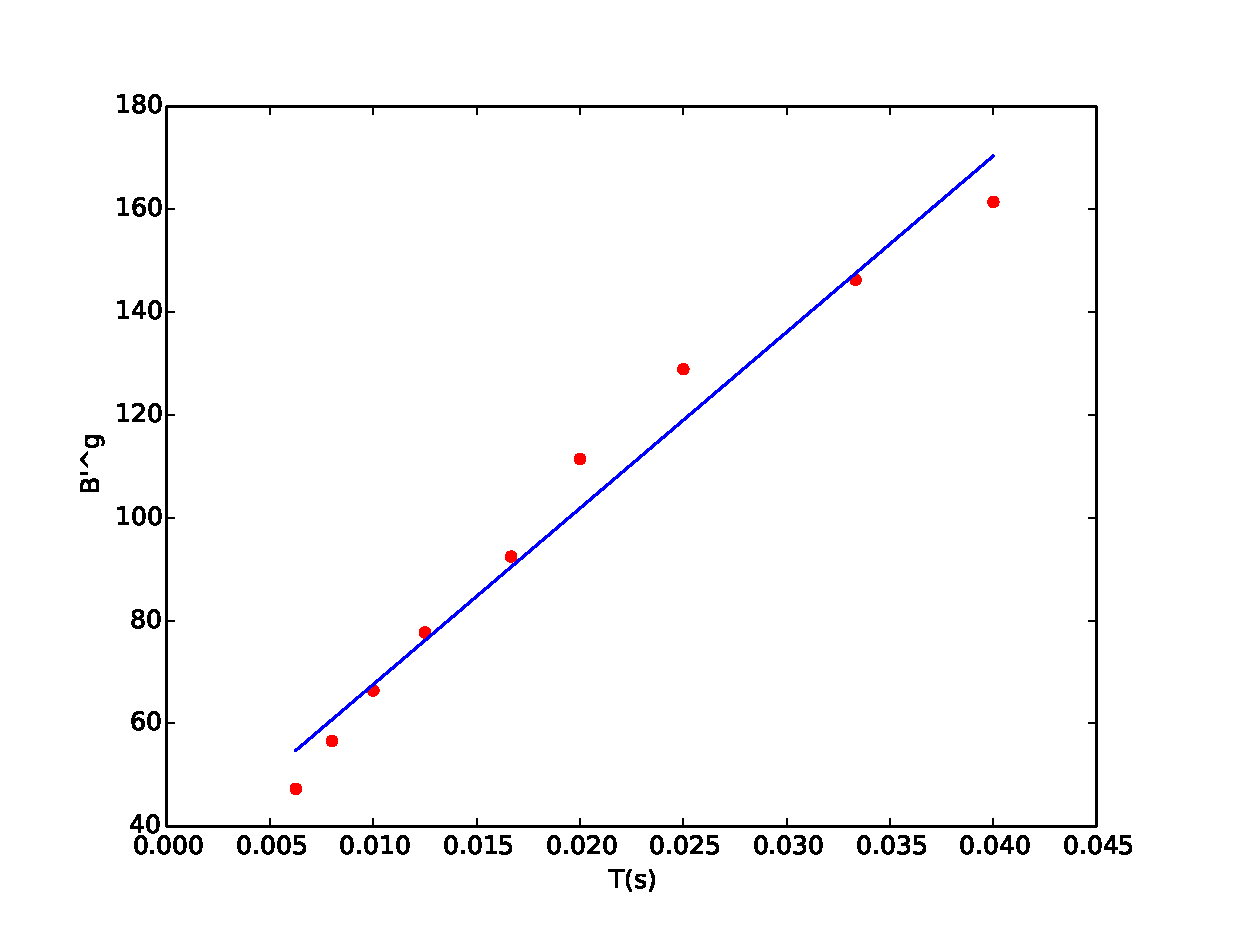
\includegraphics[width=.47\columnwidth]{images/bchannel}
}
\subfigure[Blue Channel $g=1.484$]{
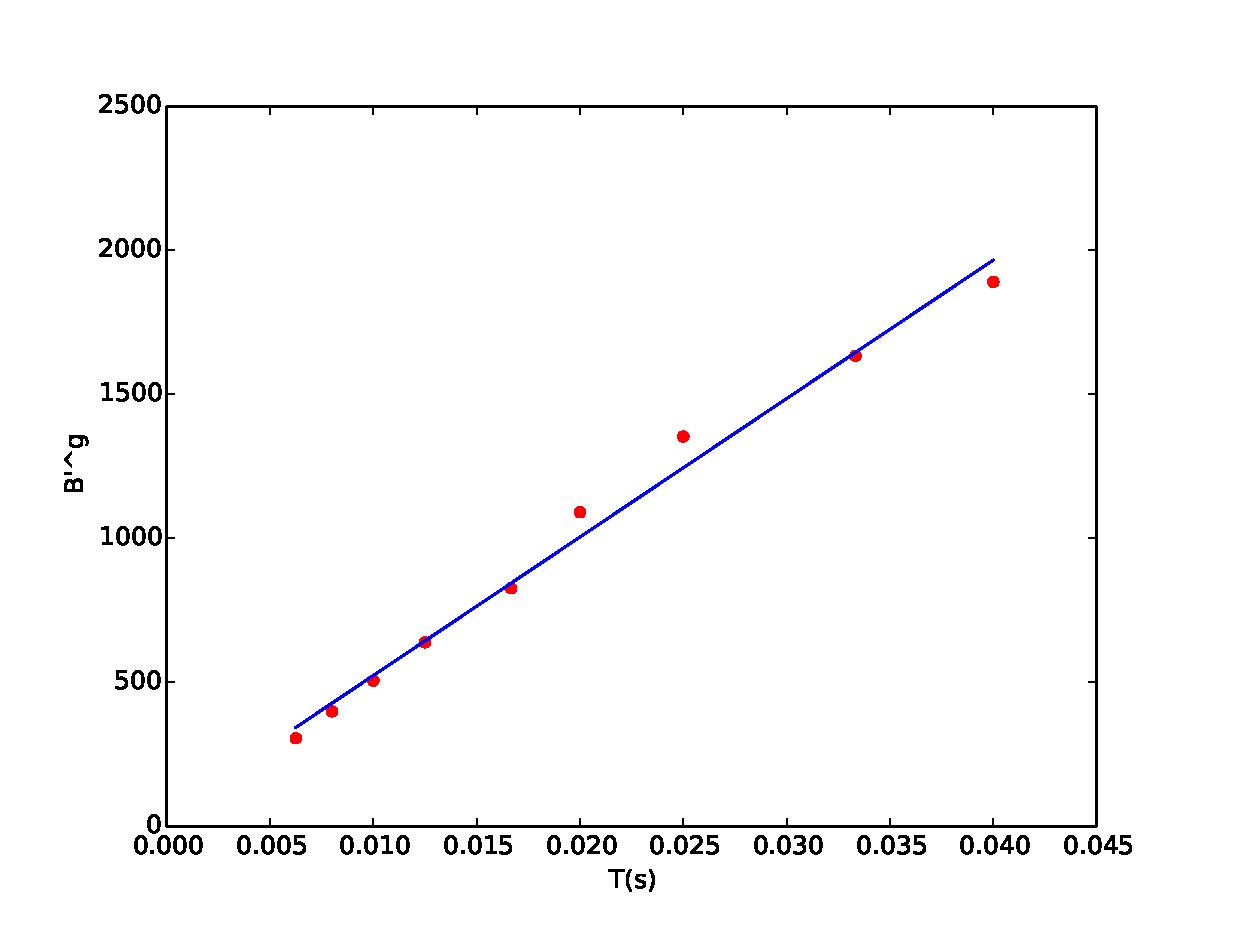
\includegraphics[width=.47\columnwidth]{images/bchannelg}
}

\caption{$B'^g(T)$ Curves}
\label{fig:samplecurves}
\end{figure}

\section{Acquire a picture stack}
\label{sec:stack}

We took another 10 pictures with the same camera and a 17mm lens. ISO was set to 400 and F-number was set to 4. The optimal exposure time was chosen to be $T_0 = 1/100s$ so that there were no saturation(ensured by the warning from camera). Then we picked another two pictures with $T_1 = 1/4s$, $T_2 = 6s$, since they got good exposures on different layers as shown in Figure \ref{fig:picturestack}. \\

Equation \ref{equ:linear} was applied to obtain the linearized pictures. To ensure the values of $B(T)$ fall in the range $[0,255]$, we divided the values of $B(T) = B'^g(T)$ by $255^{g-1}$ for each channel. The result is also shown in Figure \ref{fig:picturestack}.

\begin{figure}[t]
\centering
\subfigure[Picture with $T=1/100s$]{
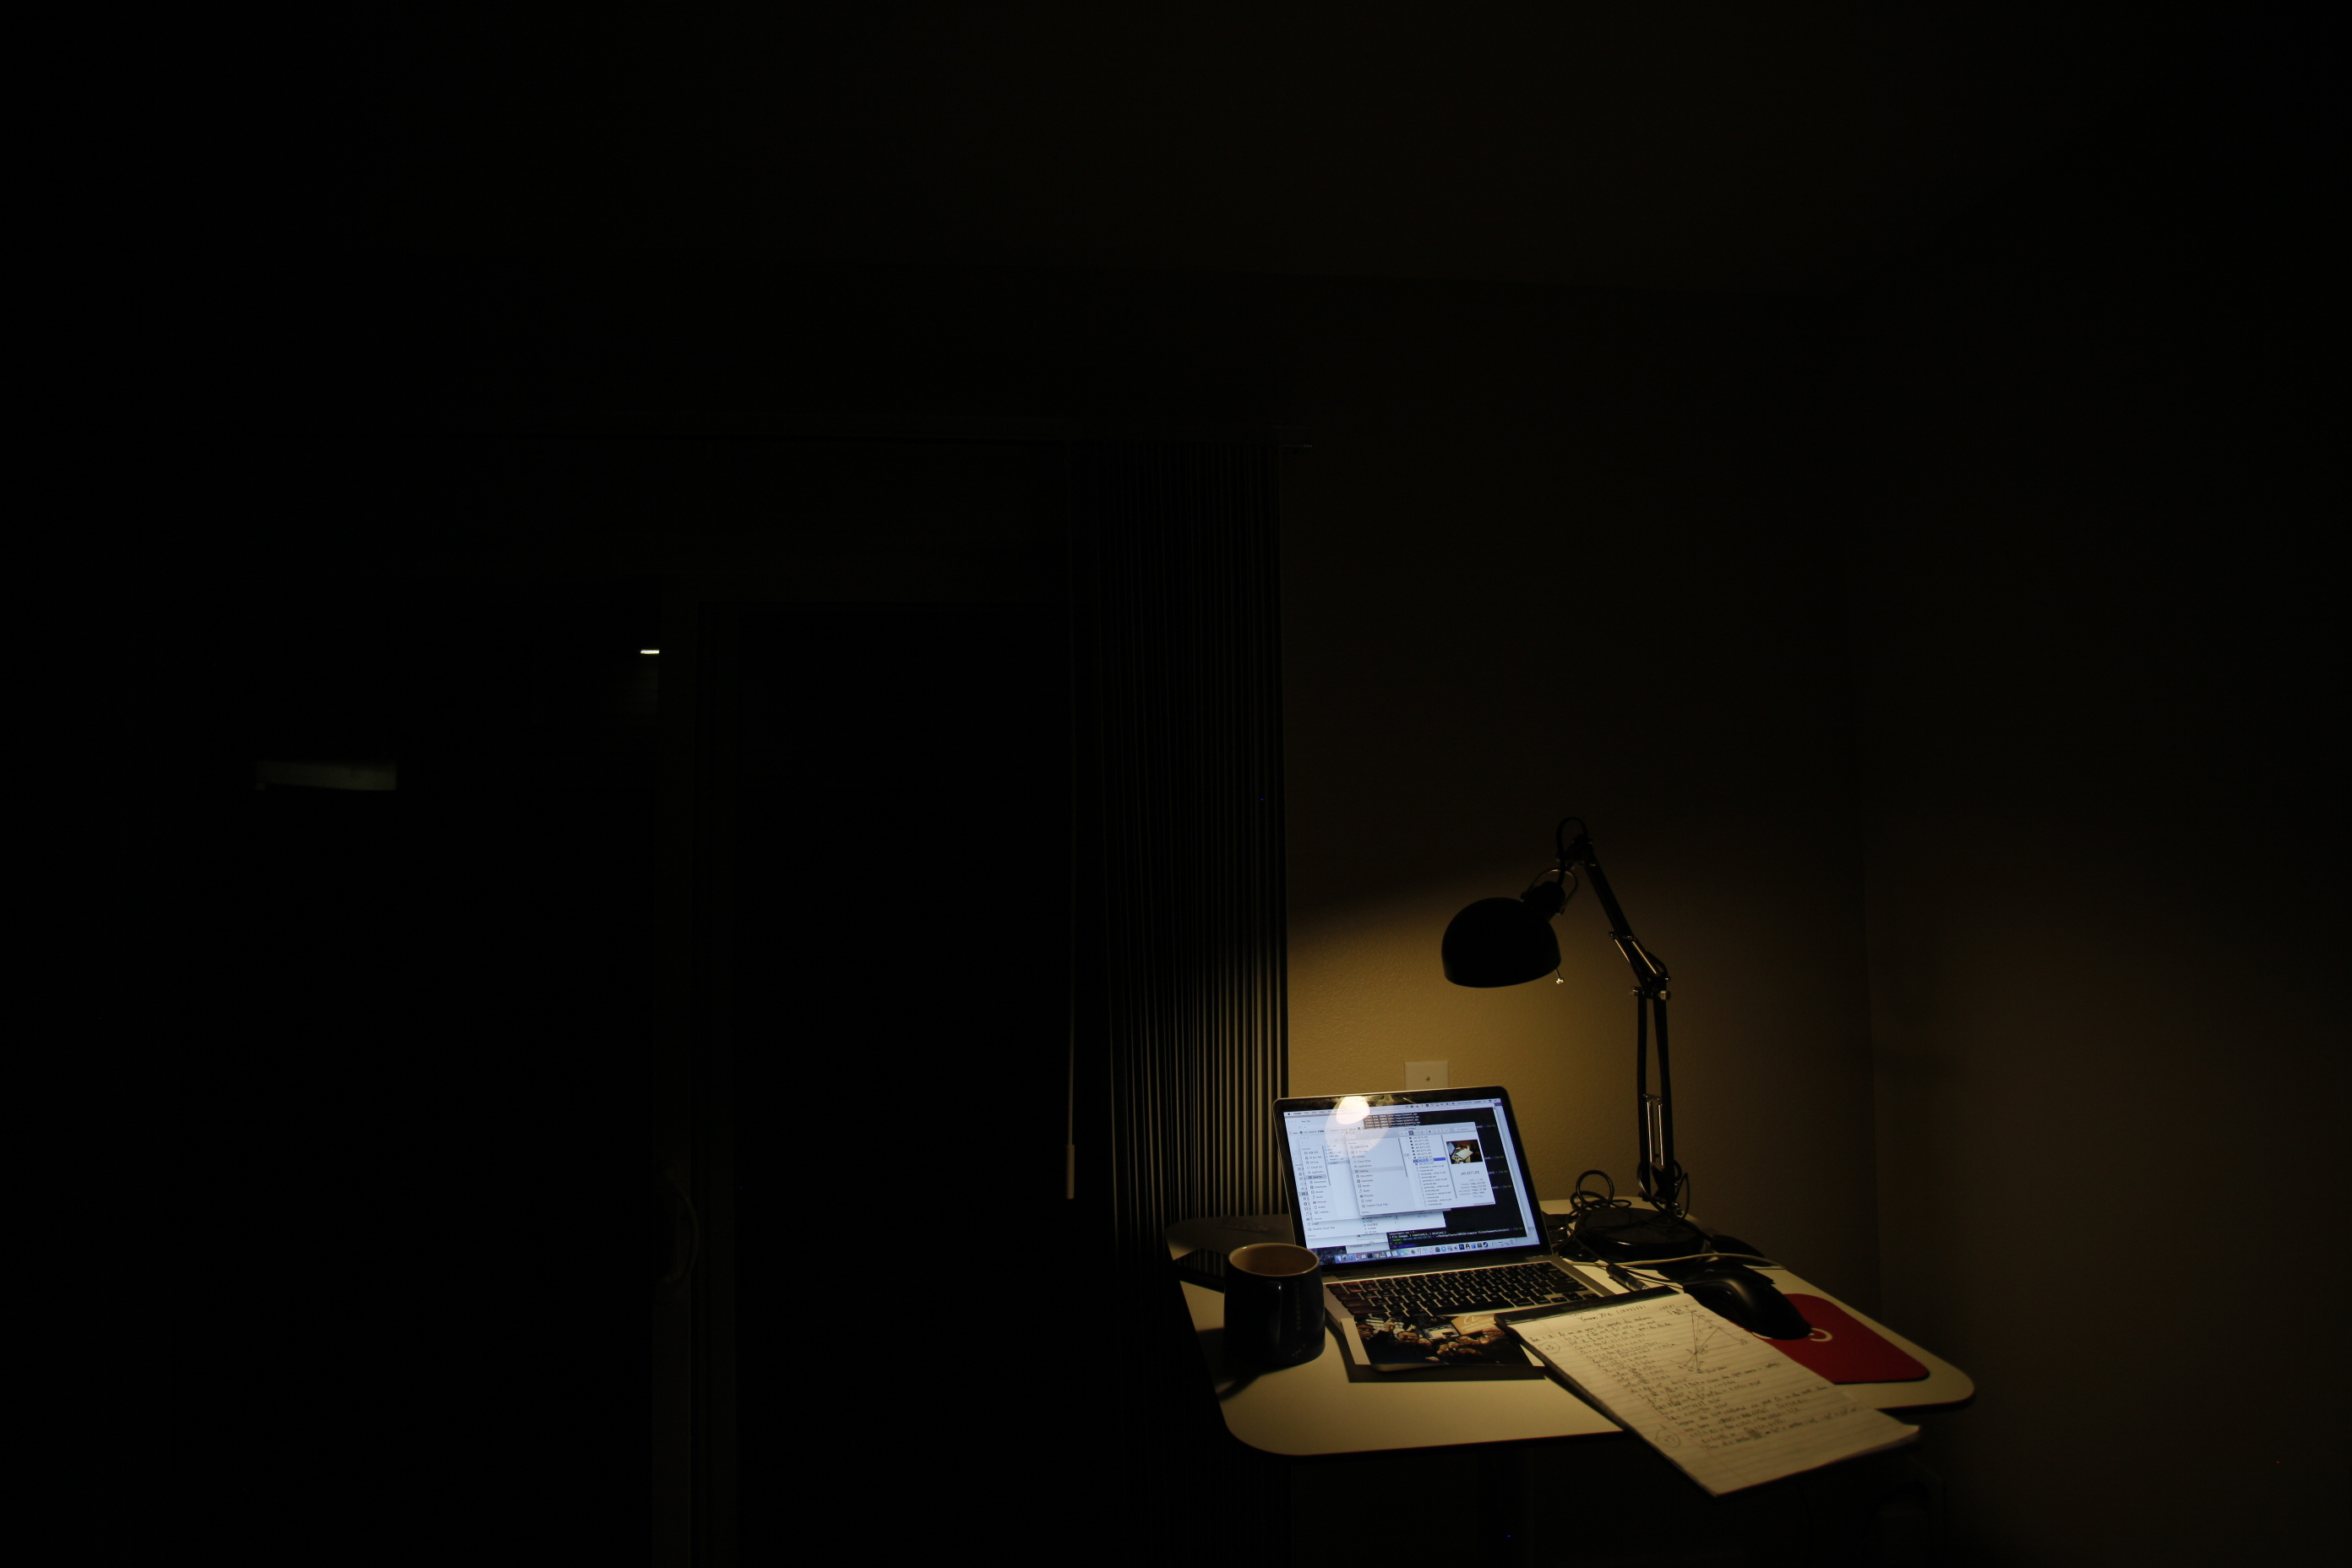
\includegraphics[width=.47\columnwidth]{images/hdr/_MG_6295}
}
\subfigure[Linearized (a)]{
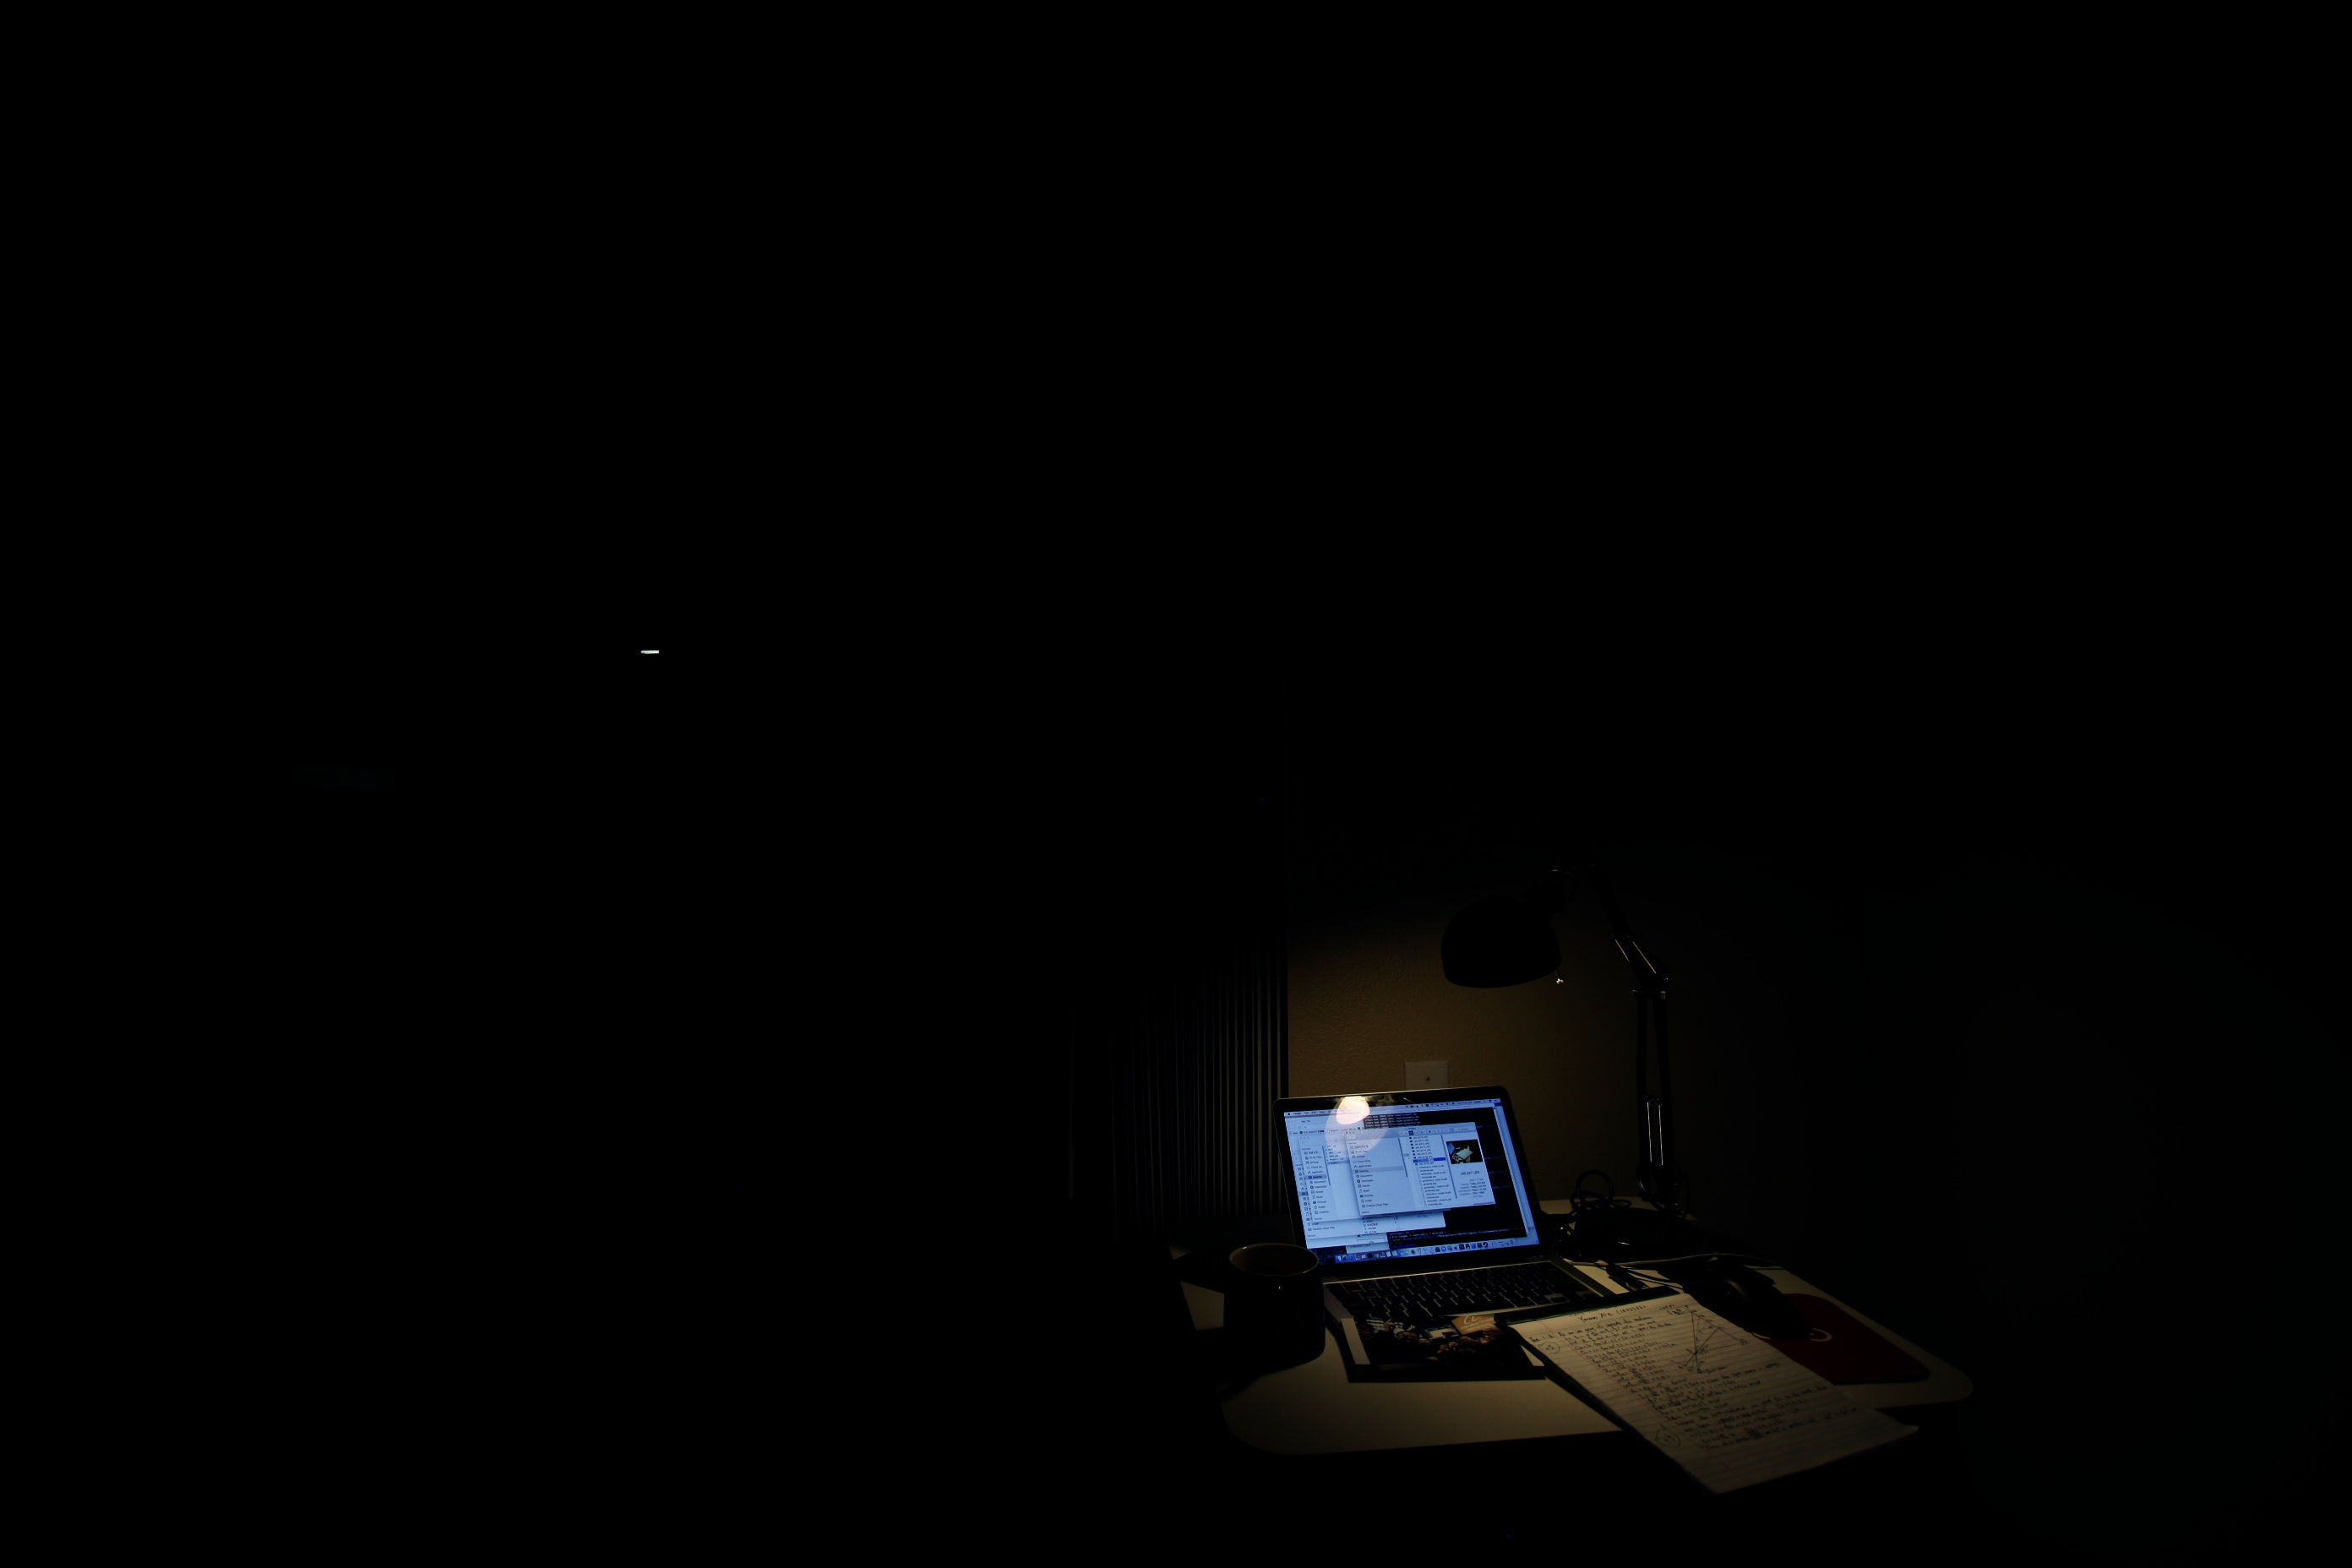
\includegraphics[width=.47\columnwidth]{images/hdr/simple_linear/_MG_6295}
}

\subfigure[Picture with $T=1/4s$]{
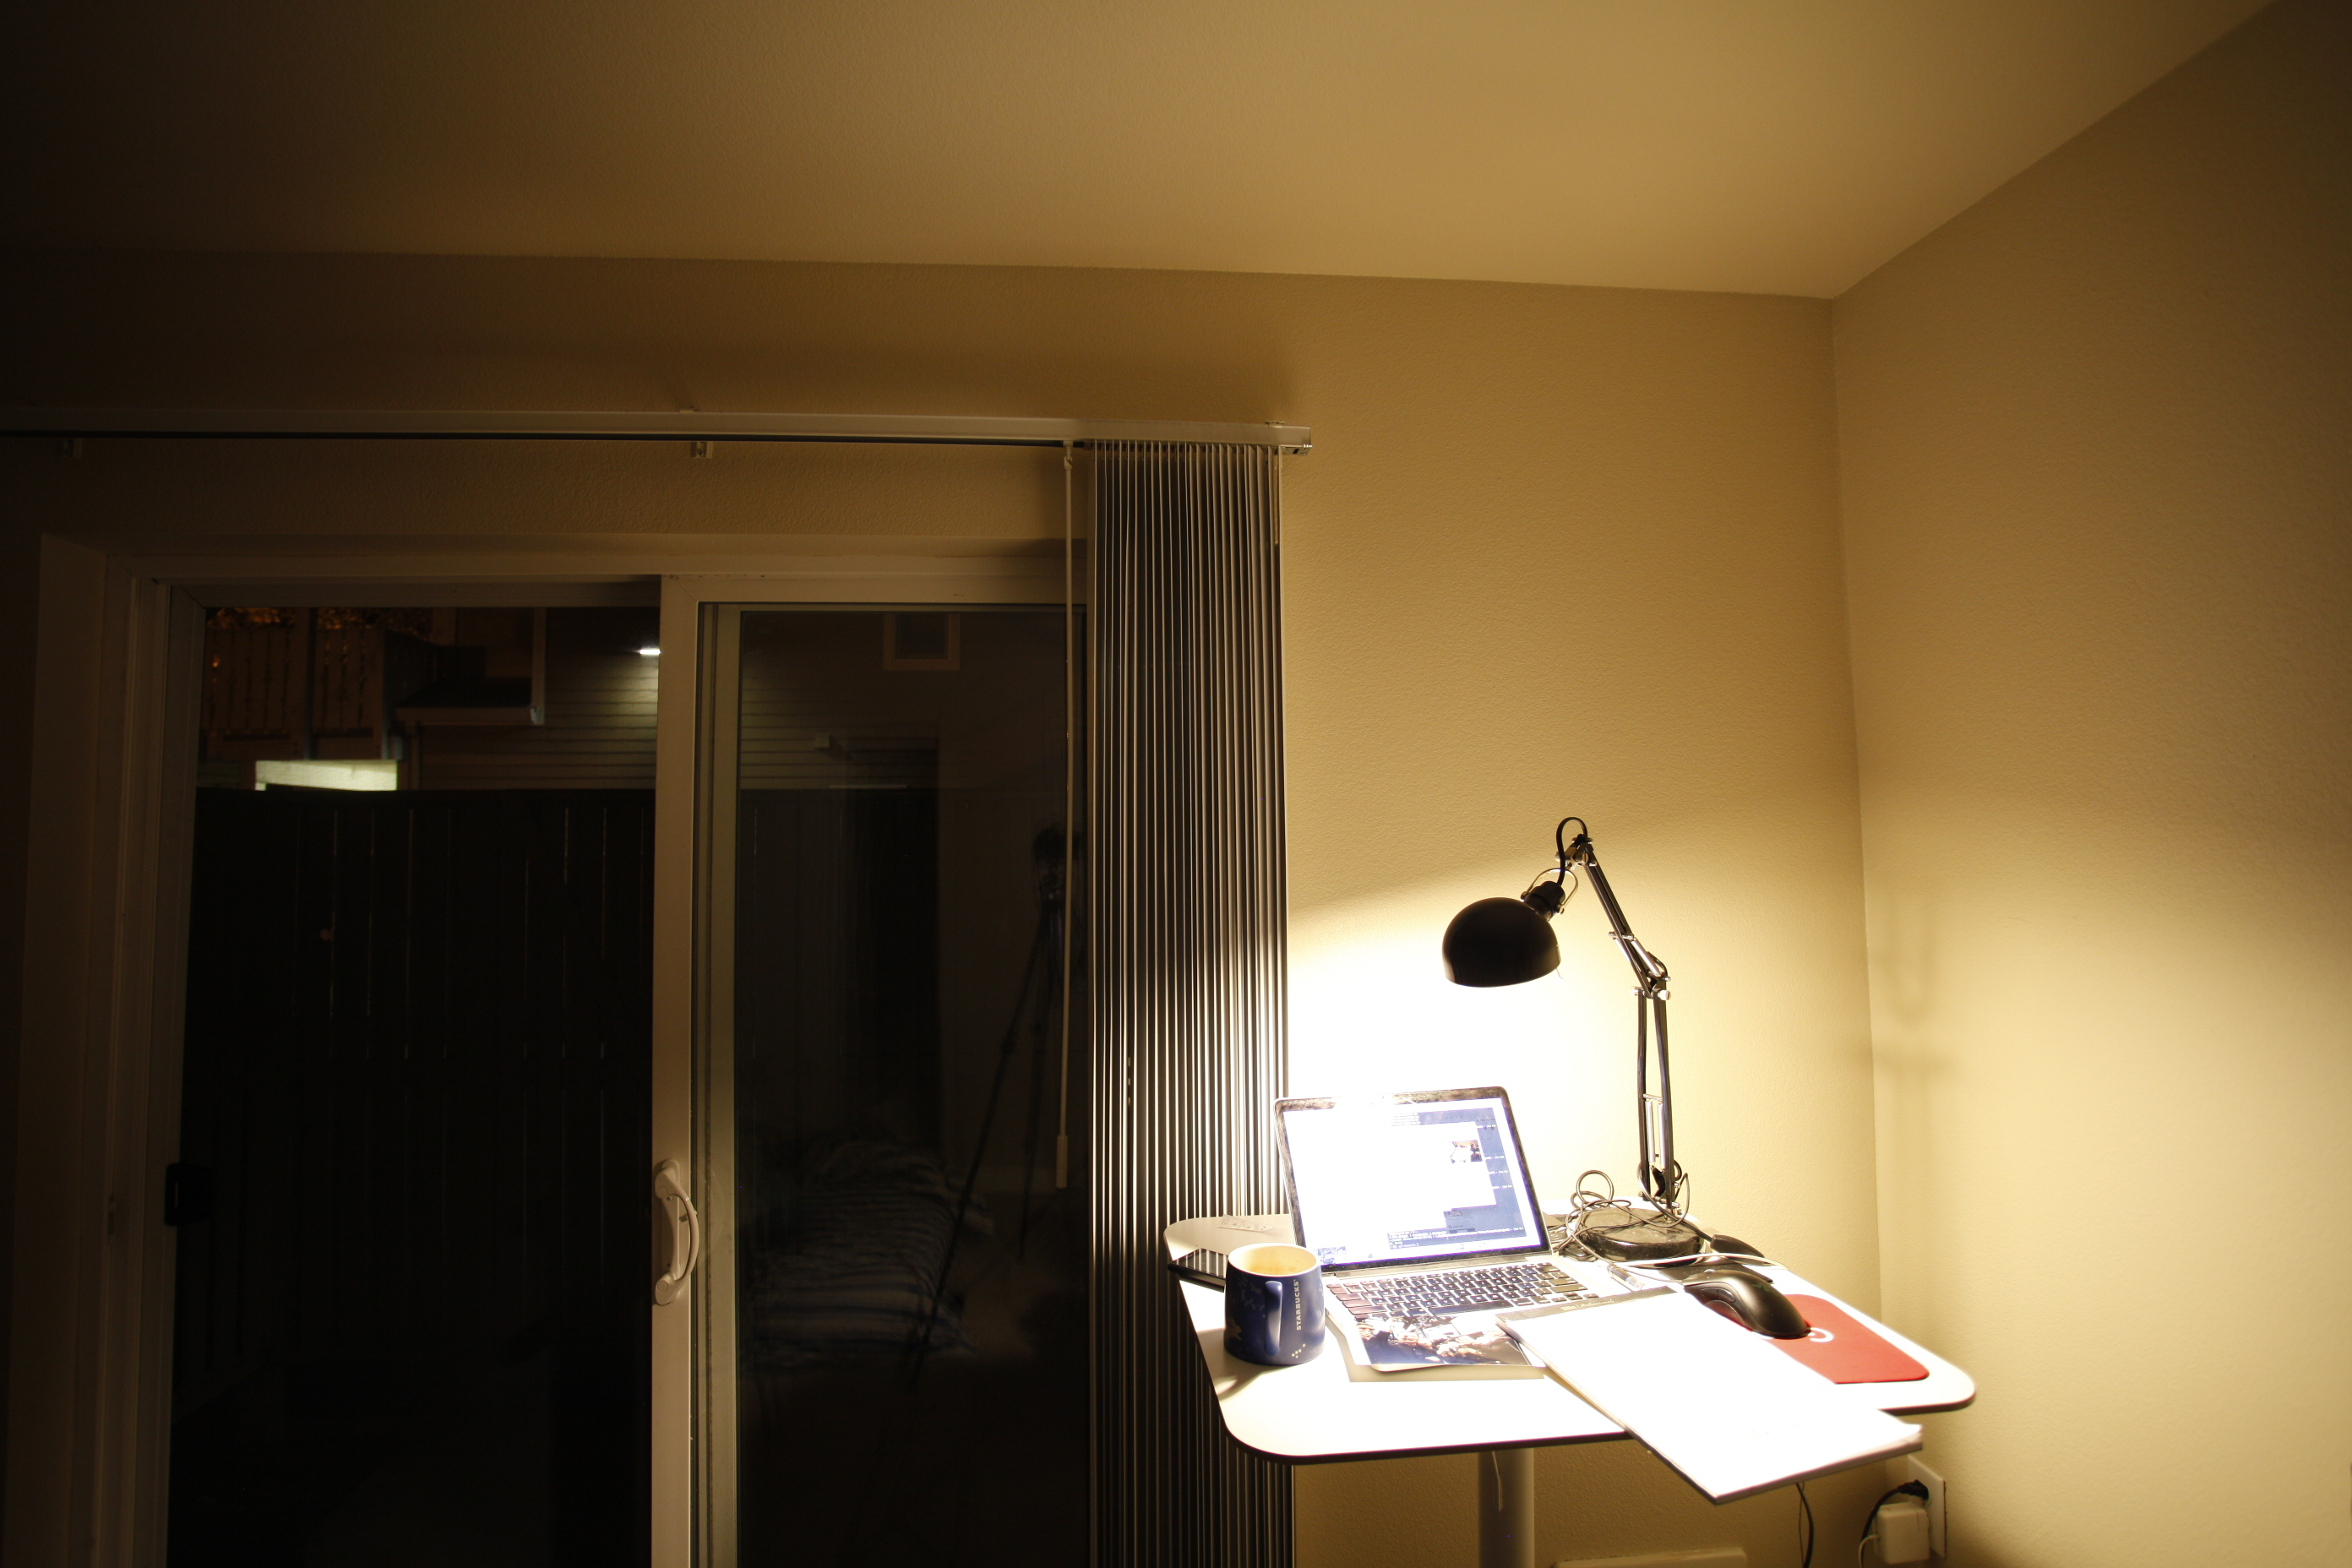
\includegraphics[width=.47\columnwidth]{images/hdr/_MG_6298}
}
\subfigure[Linearized (c)]{
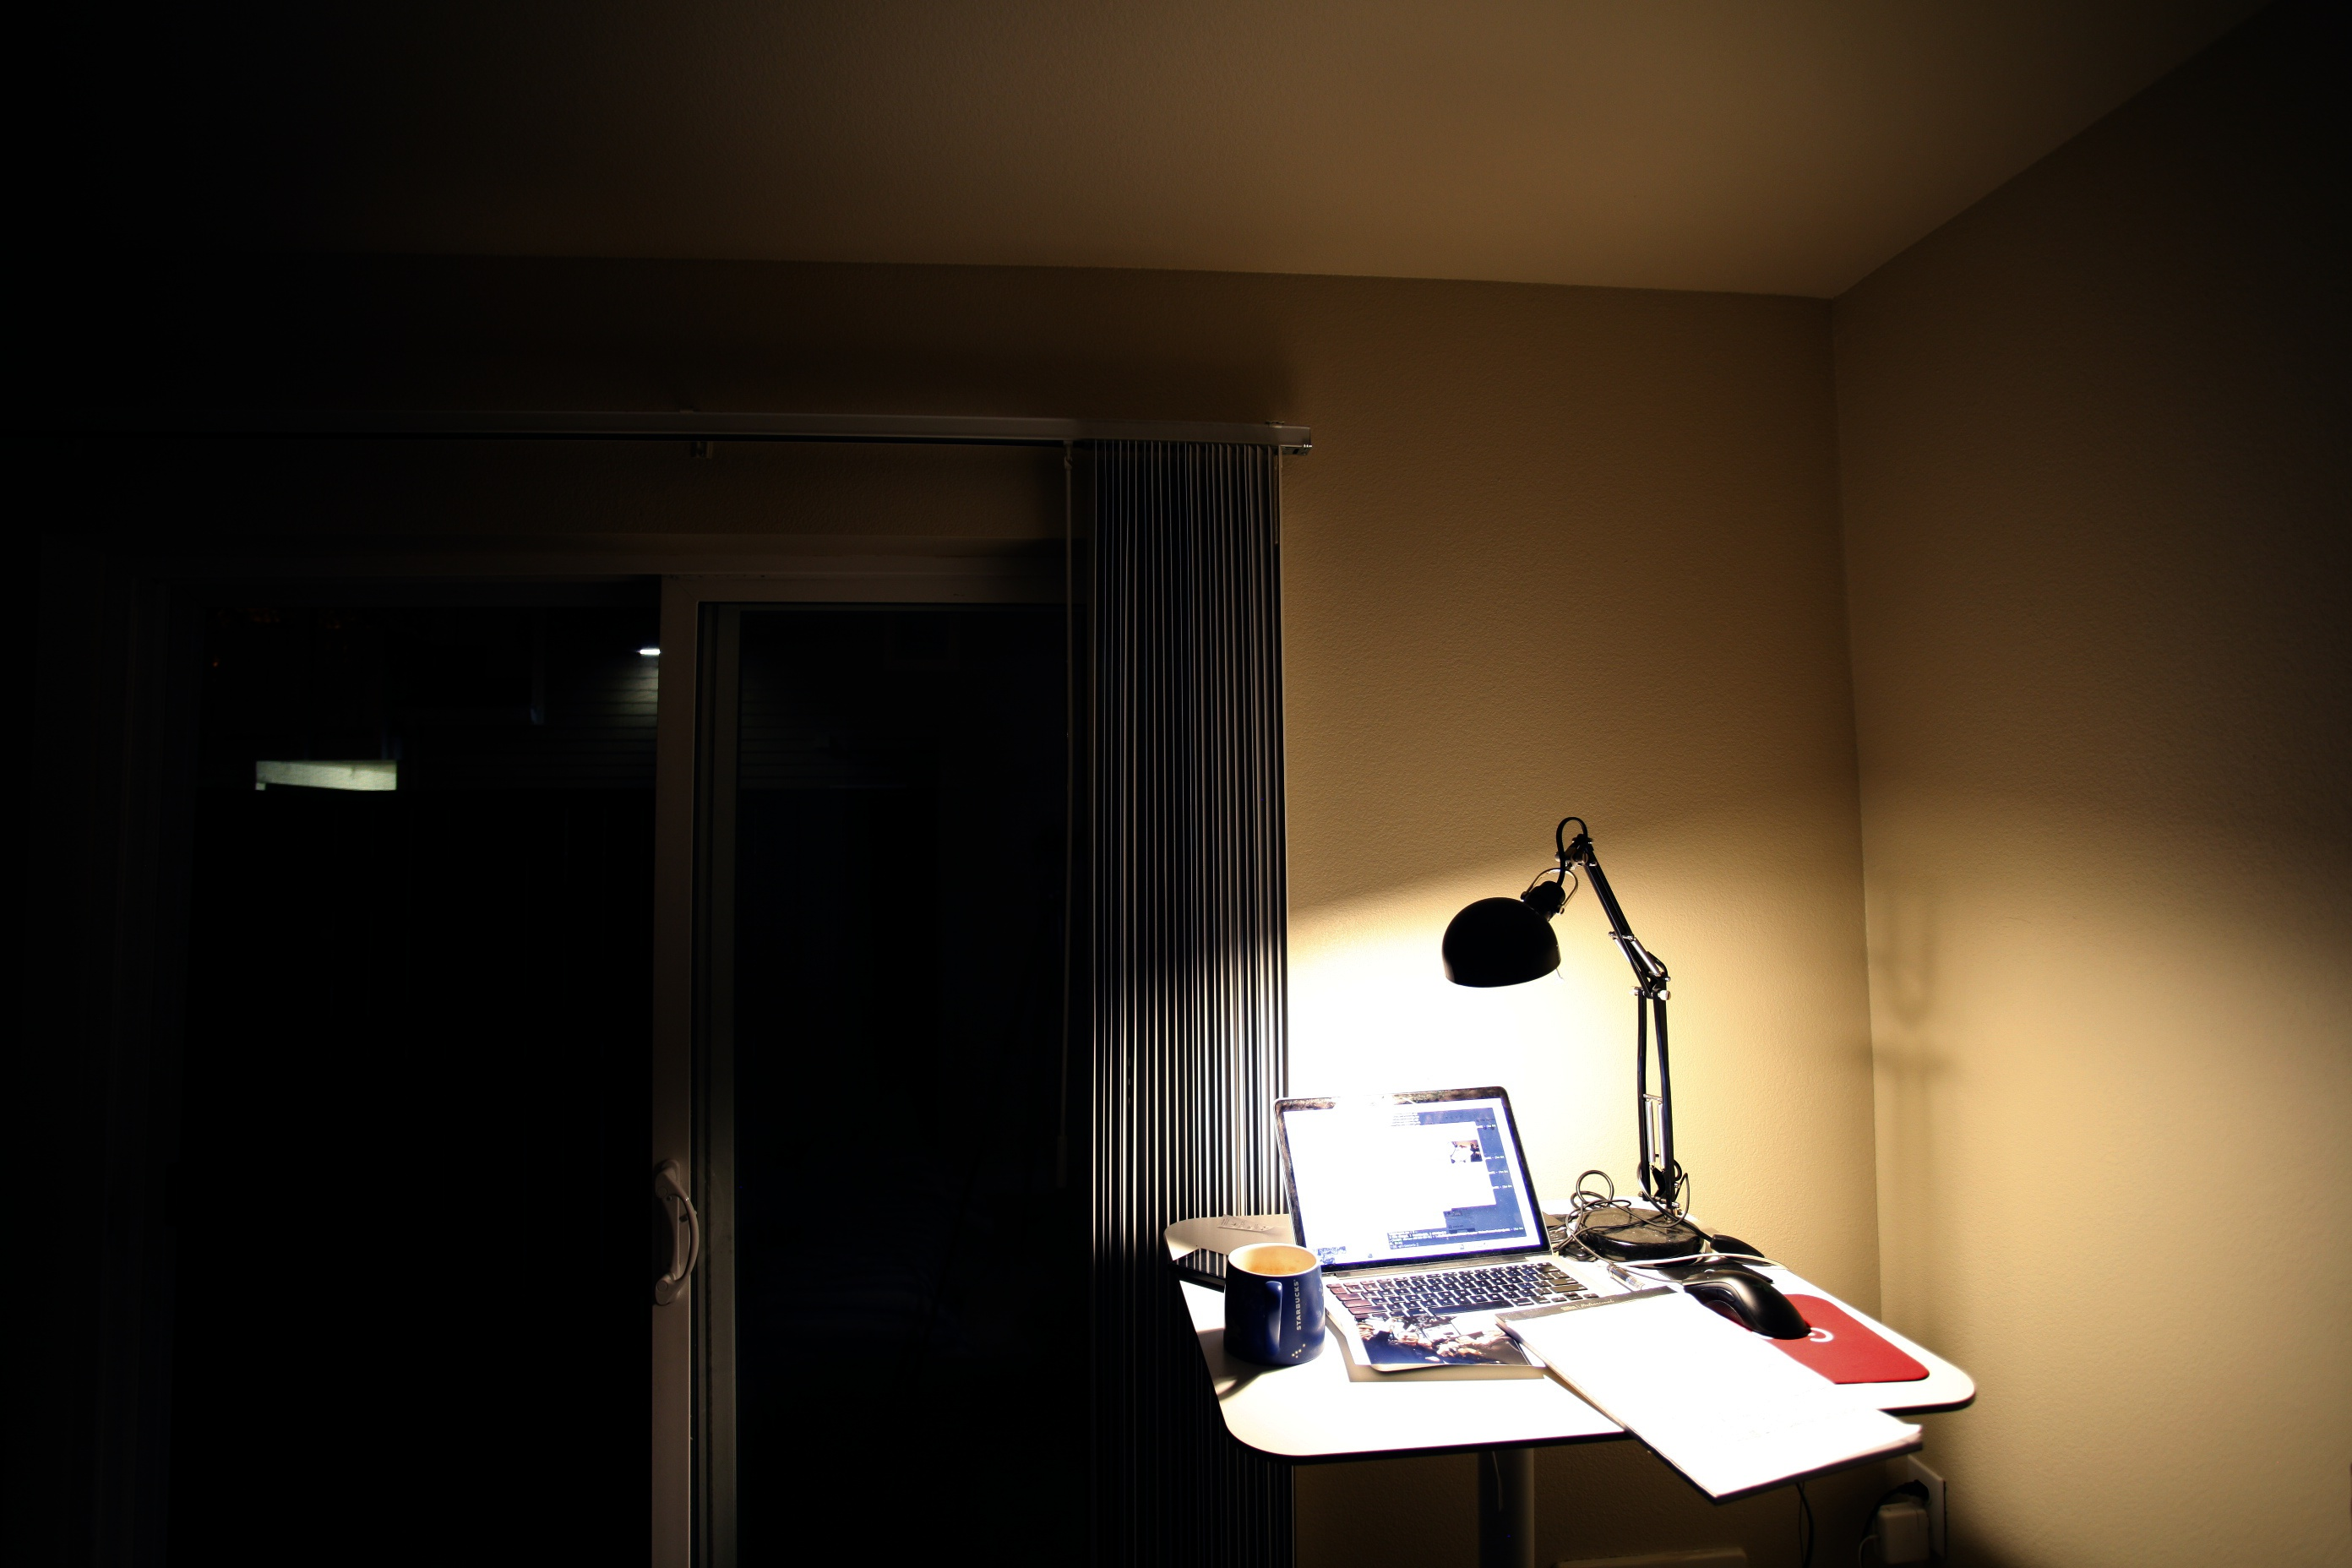
\includegraphics[width=.47\columnwidth]{images/hdr/simple_linear/_MG_6298}
}

\subfigure[Picture with $T=6s$]{

\includegraphics[width=.47\columnwidth]{images/hdr/_MG_6301}
}
\subfigure[Linearized (e)]{

\includegraphics[width=.47\columnwidth]{images/hdr/simple_linear/_MG_6301}
}

\caption{Picture Stack}
\label{fig:picturestack}
\end{figure} 

\section{Create composite image}
\label{sec:create}

\section{Reproduce composite image}
\label{sec:reproduce}

\section{Acknowledgment}
We did all the project together. However, Ziqiang Wang is mainly responsible for
Section \ref{sec:create} and Section \ref{sec:reproduce} while Yanan Xie is responsible for the rest parts of this project including providing his professional photography devices.\\

Thanks to \LaTeX\ for providing such a great document preparation system. And many appreciates to the authors of Python, numpy, sklearn, OpenCV and matplotlib.\\



\end{document}
